\documentclass[11pt]{article}
\usepackage{isma2018}

% Enter further packages required for your manuscript below.
\usepackage{graphicx}
\usepackage{amsmath}
\usepackage{amsfonts} %potrzebne do \mathbb{S}
\usepackage{amssymb}
\newcommand{\D}{\displaystyle}
\usepackage[numbers,square,sort&compress]{natbib}

%%%%%%%%%%%%%%%%%%%%%%%%%%%%%%%%%%%%%%%%%%%%%%%%%%%%%%%%%%%%%%%%%%%
% The "hyperref" package may be used in conjunction with PDFLatex %
% to add document information to the generated PDF file. Please,  %
% fill out the same title, author(s) and keywords as on the paper %
% submission form. Note, that the "hypperref" package should be   %
% loaded as the last.                                             %
%                                                                 %
% If you are not using PDFLatex, delete or comment the following  %
% lines. In that case, the conference secretary will add the      %
% document information to your PDF file.                          %
%%%%%%%%%%%%%%%%%%%%%%%%%%%%%%%%%%%%%%%%%%%%%%%%%%%%%%%%%%%%%%%%%%%

\usepackage[pdftex]{hyperref}
\usepackage{color}

\hypersetup{a4paper = true,
	pdfpagemode = None,
	pdfstartview  = FitH,
	citebordercolor = 1 1 1,
	filebordercolor = 1 1 1,
	linkbordercolor = 1 1 1,
	urlbordercolor = 1 1 1}
\hypersetup{pdftitle  = {Manuscript preparation instructions},
	pdfauthor = {P. Kruczek},
	pdfkeywords = {ISMA2018, USD2018, template}}

\title{Multi-fault diagnosis based on bi-frequency cyclostationary maps clustering}

\author{\textbf{P. Kruczek $^1$, J. Wodecki $^1$, A. Wy{\l}oma{\'n}ska $^1$, R. Zimroz $^2$, K. Gryllias $^3^,$ $^4$
} \\
  $^1$ KGHM Cuprum Ltd, R \& D Centre, \\
  Sikorskiego 2-8, 53-659 Wroclaw, Poland, \\
  e-mail: \textbf{p.kruczek@cuprum.wroc.pl} 
% Uncomment this block to add multiple (different) affiliations.
 \\ [3mm]
 $^2$ Faculty of Geoengineering, Mining and Geology, Wroc{\l}aw University of Science and Technology, \\
 Na Grobli 15, 50-421 Wroclaw, Poland
 \\ [3mm]
 $^3$ KU Leuven, Department of Mechanical Engineering, \\
 Celestijnenlaan 300 B, B-3001, Leuven, Belgium 
 \\[3mm]
$^4$ Dynamics of Mechanical and Mechatronic Systems, Flanders Make, Belgium
  }

\date{}

\begin{document}

\abstract{During the last decade, condition monitoring of rotating machinery is a field of intensive research being closely related to the industry. Therefore a plethora of different approaches have been proposed focusing towards the early detection and diagnosis of faults. Among others, some of the most powerful diagnostic tools are based on the exploitation of the cyclostationary properties of the signals, captured over a rotating machine. In this paper an advanced signal processing diagnostic tool is introduced based on the recently proposed Cyclic Spectral Coherence (CSC). The Cyclic Spectral Coherence is represented in a 3D bi-frequency map, providing information about the modulation frequencies which are presented in vibrations signals. The characteristic fault frequencies related to the local damage can be identified directly in those bi-frequency maps, however usually their interpretation is a challenging task. The 3D maps can be further integrated on the whole frequency band or on optimally selected bands leading to 2D vectors, which are  equivalent to the classical Squared Envelope Spectrum (SES). Fault diagnosis is more challenging in the case of complex signals, such as vibration signals captured on heavy duty mining machinery, which usually suffer from high noise contamination. The captured signals often contain many different sources of noise and more than one fault components. In this case, the detection and interpretation of the fault components on the spectrum resulted by the integration of a 3D map could be very challenging for a non-expert. Therefore a new methodology is proposed, which focuses on the separation of the information linked to different types of defects by applying tools for clustering on the bi-frequency CSC map. Each vector corresponding to each modulation frequency (alpha axis) including all the carrier frequencies is considered as a single point at the m-dimensional space. The clustering tools create clusters which group the similar vectors. As a result, each cluster will contain the separated/isolated information of each fault while one cluster will include the vectors where the diagnostic information is present. Moreover a CSC map will be recreated based on each cluster and the integration over the whole carrier frequency band will lead to a clear Square Envelop Spectrum which will include only one type of defect. The methodology is tested and evaluated on simulated signals and on real industrial signals recorder on heavy duty machines located in an underground mine.}

\maketitle

\section{Introduction}

Modern condition monitoring techniques are able to diagnose damages at early stage, in complex machines, under varying speed/load condition, in presence of heavy, impulsive noise, \cite{wylomanska2017application,borghesani2013new,schmidt2018novelty,gryllias2018application,javorskyj2016periodically}. In \cite{kruczek2017cyclic} the cyclic source extraction method from complex vibration signal was presented. The application of the Schur filter for local damage detection in machinery was illustrated in \cite{makowski2014new}.
However, to face such challenging tasks, researchers are developing more and more advanced signal processing techniques and diagnostic procedures \cite{wylomanska2016impulsive,hu2016development,michalak2017application}. Therefore, they are  complex and  require an expert to interpret results. Indeed, it is a typical obstacle  for most of 3-dimensional representations of the signal, namely time-frequency map, bi-spectrum or Cyclic Spectral Coherence \cite{kruczek2017multiple}. Obviously, the final result depends on level of complexity of both: method and analyzed signal. 
The real industrial signals are complex and  contaminated . Therefore, experts prefer to use the methods, which are easy to interpret. There is a need for an automatic methods for damage detection \cite{wodecki2018optimal}. In order to avoid such a situation, we propose an automatic procedure for understanding such 3D map and providing simple picture commonly presented in textbooks. In some sense it could be considered as source separation, however in bi-frequency domain. 

 Let us recall that the Cyclic Spectral Coherence is  a 3D bi-frequency map, providing information about the modulation and carrier frequencies, which are present in vibrations signals. Moreover, one can observe  characteristic fault frequencies related to the local damage  in CSC. Furthermore, these 3D maps can be  integrated on the whole frequency band or on optimally selected bands leading to 2D vectors which are considered equivalent to the classical squared envelope spectrum.
 However, in case of heavy duty machine with multiple faults located at different shaft (with different speed) it might happen that fault related patter in CSC map integrated to 2D envelope spectrum is hard to identify. By application of proposed clustering techniques one could separate content related to given fault, so finally instead of one figure with multiple faults one could obtain several  figures with single fault. In our opinion it would be much easier to interpret and analyze. 

In this paper we propose complete procedure how to automatically process 3D CSC map with two faults with different locations (i.e. fault frequencies) and different carrier frequencies. The procedure has been applied to real signal from two stage gearbox operated in heavy duty drive unit used in mining applications. We will show, that source separation in bi-frequency domain is possible after integration of new map to envelope spectrum (ES) \cite{randall2001relationship}. The structure of ES is much clear and allows to easily identify damage. Clustering algorithm used here is Expectation Maximization \cite{dempster1977maximum, kaufman2009finding} algorithm. However, we are focused on simple decision making procedure for condition monitoring.  

The paper is organized as follow. In the next section the proposed methodology is described. The CSC and EM methods are presented and the  clustering of the map is explained. In section \ref{sec:application} the application of the method to real data is presented. Last section is the summary of the performed research.



\section{Methodology}
Proposed procedure is a combination of three techniques, namely CSC representation, clustering via EM algorithm, integration of obtained new CSC maps (for each cluster separately). In fact all these techniques are well-known, however their combination is novel approach for multiple fault case and provides promising results. In this section we are going to recall the  definitions and main properties of the proposed methodology. Furthermore, their fusion is illustrated and described. 

\subsection{Cyclic spectral coherence}
Cyclic spectral coherence  is a function, which depends on the modulation and carrier frequency. It was introduced by
 Antoni in 2007~\cite{antoni2007cyclic}. It is a powerful tool to indicate the cyclostationary property of the signal.  Firstly, we recall the cyclic power spectrum (CPS) $S_X(f;\alpha)$ of the signal $\mathbf{x}$:
\begin{equation}
\label{eq:CPS}
S_X(f;\alpha)=\lim_{L\to \infty}\D{1\over L}\mathbb{E}\left(\mathcal{F}_{\mathbf{x},L}(f+\D{\alpha \over 2})\overline{\mathcal{F}_{\mathbf{x},L}(f-\D{\alpha \over 2})}\right),
\end{equation}
where $\mathcal{F}_{\mathbf{x},L}(f)$ is Fourier transform of the signal $\mathbf{x}$ calculated on interval of length $L$.
CPS is used to measure the spectral dependency in the analyzed signal and it relies on modulation ($\alpha$) and carrier ($f$) frequencies. It is expected CPS satisfy $\left|S_X(f;\alpha)\right|>0$ for cyclostationary signal for some $\alpha\neq 0$. Finally, we can formulated the definition of CSC:
 ~\cite{antoni2007cyclic}:
\begin{equation}
\label{eq:SC}
SC(f;\alpha)=\left|\gamma_X(f;\alpha)\right|^{2}=\D { \left|S_X(f;\alpha)\right|^2 \over S_X(f+\D{\alpha \over 2};0)S_X(f-\D{\alpha \over 2};0)}.
\end{equation}
It is a normalized CPS, thus its value is in the interval $(0,1)$. It is expected that, CSC describe the spectral cyclic autocorrelation of the signal. Therefore, it can be used as a cyclostationary indicator. Once the $\left|\gamma_X(f;\alpha)\right|^{2}$ is significantly higher than 0, then signal has cyclostationary property for modulation frequency $T=1/\alpha$ and carrier frequency $f$.
\\
The estimation of CSC can be directly performed using CPS estimator. Thus the following formula is obtained:
\begin{equation}
\left|\hat{\gamma}_X(f;\alpha)\right|^{2}=\D { \left|\hat{S}_X(f;\alpha)\right|^2 \over \hat{S}_X(f+\D{\alpha \over 2};0)\hat{S}_X(f-\D{\alpha \over 2};0)},
\end{equation} 
where $\hat{S}_X(f;\alpha)$ is an estimator of the CPS.
It is worth mentioning that, there are many different methods for estimation of CPS \cite{antoni2007cyclic2}. In our study we used the Welch method.

\subsection{Expectation - maximization}
In this section the expectation-maximization  method, for clustering the data, is described \cite{sundberg1974maximum,dempster1977maximum}. 
Expectation – Maximization  is an iterative optimization method for estimation of unknown parameters for given measurement data $X$. EM is particularly useful for separating mixtures of Gaussian distributions (or any other) over the considered feature space. It consists of two main steps: Expectation (E-step) and Maximization (M-step), that are iterated until convergence. 

Firstly, let us assume  that we have observed the following N data points in a $D$-dimensional space \newline
$X=\{\overrightarrow{x}_1,\overrightarrow{x}_2,\dots \overrightarrow{x}_N\}$. Furthermore, $N$ points are drawn from $D$-dimensional Gaussian distribution. The $l$-th distribution characterized by the parameters $\theta_l=\{\overrightarrow{\mu}_l,\Sigma_l\}$, where $\overrightarrow{\mu}_l$ is the $D$-dimensional mean and $\Sigma_l$ is the covariance matrix. Therefore, we  assign a prior probability $\alpha_l$ with the $l$-th Gaussian, where $\sum_{l=1}^N \alpha_l=1$.

% Furthermore, it is assumed that, the drawn Gaussian distribution for given element $X$ is unknown. However, it is known that each element of the dataset $X$ is characterized by the following mixture probability density function:
% \begin{equation}
%     p(\overrightarrow{x}|\Theta)=\sum_{l=1}^K \alpha_l p_l (\overrightarrow{x}|\theta_l),
% \end{equation}
% Where $\Theta$ represents all the parameters involved in the description of the mixture:
% \begin{equation}
%     \Theta=(\alpha_1,\alpha_2,\dots,\alpha_K;\theta_1,\theta_2,\dots,\theta_K).
% \end{equation}
% As it is expected, the $l$-th Gaussian in the mixture is given by:
% \begin{equation}
% \label{eq:distribution1}
%     p(\overrightarrow{x}|\theta_l)=\frac{1}{(2\pi)^{d/2}|\Sigma_l|^{1/2}}\exp{\left(-\frac{1}{2}(\overrightarrow{x}-\overrightarrow{\mu}_l)^T\Sigma_l^{-1}(\overrightarrow{x}-\overrightarrow{\mu}_l)\right)}
% \end{equation}
% If we assume that the $N$ observations in $X$ are independent, we can write the following expression for the probability distribution for all of the observations in $X$:
% \begin{equation}
% \label{eq:distribution2}
%      p(\overrightarrow{x}|\Theta)=\prod_{i=1}^Np(\overrightarrow{x}_i|\Theta)=\prod_{i=1}^N\left( \sum_{l=1}^K\alpha_lp_l(\overrightarrow{x}_i|\theta_l) \right).
% \end{equation}
% Substituting the individual Gaussians from Equation (\ref{eq:distribution1}) in (\ref{eq:distribution2}), we can write  the probability distribution for all of our dataset:
% \begin{equation}
% \label{eq:distribution3}
%     p(\overrightarrow{x}|\Theta)=\prod_{i=1}^N\left( \sum_{l=1}^K\alpha_l\frac{1}{(2\pi)^{d/2}|\Sigma_l|^{1/2}}\exp{\left(-\frac{1}{2}(\overrightarrow{x}-\overrightarrow{\mu}_l)^T\Sigma_l^{-1}(\overrightarrow{x}-\overrightarrow{\mu}_l)\right)} \right).
% \end{equation}
% If the parameter set $\theta$ is known, then $ p(\overrightarrow{x}|\Theta)$ is a probability distribution for the dataset $X$. However, the main  goal is to estimate $\Theta$ from a given set of observations $X=\{\overrightarrow{x}_1,\overrightarrow{x}_2,\dots \overrightarrow{x}_N\}$, thus it is prefered to consider the right hand side in equation (\ref{eq:distribution3}) as the likelihood that informs how likely the known observations in $X$ are for candidate values for the elements of $\Theta$. To make this fact more explicit, we rewrite equation (\ref{eq:distribution3}) as:
    
%     \begin{equation}
%         L(\Theta|X)=\prod_{i=1}^N\left( \sum_{l=1}^K\alpha_l\frac{1}{(2\pi)^{d/2}|\Sigma_l|^{1/2}}\exp{\left(-\frac{1}{2}(\overrightarrow{x}-\overrightarrow{\mu}_l)^T\Sigma_l^{-1}(\overrightarrow{x}-\overrightarrow{\mu}_l)\right)} \right)
%     \end{equation}
% Our goal is to construct a Maximum Likelihood estimate for $\Theta$ by seeking $\Theta^*$ that maximizes the log-likelihood:
% \begin{equation}
%   \Theta^*=\textrm{argmax}_{\Theta}\ln(L(\Theta|X)).
% \end{equation}
% Then 
% % \begin{align}
% %     B'_m(x)&=\sum_k \binom{m}{k}(m-k)B_kx^{m-k-1} 
% %     =\nonumber\\
% %     &=
% %     m\sum_k \binom{m-1}{k}B_k x^{m-1-k}
% %     =\nonumber\\
% %     &=
% %     mB_m-1(x)
% % \end{align}
% \begin{align}
%     \Theta^*=\textrm{argmax}_{\Theta}\ln\left[\prod_{i=1}^N\left( \sum_{l=1}^K\alpha_l\frac{1}{(2\pi)^{d/2}|\Sigma_l|^{1/2}}\exp{\left(-\frac{1}{2}(\overrightarrow{x}-\overrightarrow{\mu}_l)^T\Sigma_l^{-1}(\overrightarrow{x}-\overrightarrow{\mu}_l)\right)} \right)\right]\nonumber
%     \\
%     =\textrm{argmax}_{\Theta}\left[\sum_{i=1}^N\left(\ln \sum_{l=1}^K\alpha_l\frac{1}{(2\pi)^{d/2}|\Sigma_l|^{1/2}}\exp{\left(-\frac{1}{2}(\overrightarrow{x}-\overrightarrow{\mu}_l)^T\Sigma_l^{-1}(\overrightarrow{x}-\overrightarrow{\mu}_l)\right)} \right)\right]
%     \label{eq:MLE}
% \end{align}
% According to equation (\ref{eq:MLE}) it is a challenging task to determine  a $\Theta$ that maximizes the log-likelihood, because we are dealing with the logarithm of a summation of exponentials. In this case the usual convenience afforded by the fact that the logarithm of an isolated Gaussian distributions reduces to a simple quadratic form cannot help us here. This is why we need the EM algorithm.



In the first iteration algorithm has to be provided with some initial values of parameters $\Theta$. It can be done by picking random means, covariances and distribution weights, but it is a good practice to pre-estimate means $\overrightarrow{\mu}_l$  using some simpler  algorithm like k-means or hierarchical clustering, then compute covariance matrices $\Sigma_l$ basing on results of this pre-clustering, and set weights $\alpha_l$ to normalized amount of points in each cluster.
 \begin{itemize}
     \item E-step
 \end{itemize}
This step is responsible for estimation of probability that  data point $\overrightarrow{x}_i$  belongs to cluster $\theta_l$:
\begin{equation}
    p(\theta_l|\overrightarrow{x}_i)=\alpha \frac{1}{(2\pi)^{\frac{D}{2}}|\Sigma_l|^{\frac{1}{2}}}\exp\left(-\frac{1}{2}(\overrightarrow{x}_i-\overrightarrow{\mu}_l)^T\Sigma_l^{-1}(\overrightarrow{x}_i-\overrightarrow{\mu}_l)\right).
\end{equation}
    \begin{itemize}
        \item M-step
    \end{itemize}
In this step algorithm estimates the new parameters $\Theta$ of the probability distribution of each cluster for the next iteration. Firstly the mean for each cluster is computed by calculating the mean of all points in function of the relevance degree of each point:
\begin{equation}
    \mu_l(t+1)=\frac{\sum_{i=1}^N p(\theta_l|\overrightarrow{x}_i)\overrightarrow{x}_i}{\sum_{i=1}^N p(\theta_l|\overrightarrow{x}_i)}.
\end{equation}
Then covariance matrices can be computed, basing on the conditional probability of the cluster occurrence:
\begin{equation}
    \Sigma_l(t+1)=\frac{\sum_{i=1}^N p(\theta_l|\overrightarrow{x}_i)(\overrightarrow{x}_i-\overrightarrow{\mu}_l(t))^T(\overrightarrow{x}_i-\overrightarrow{\mu}_l(t))}{\sum_{i=1}^N p(\theta_l|\overrightarrow{x}_i)}.
\end{equation}
At the end of the M-step the probability of occurrence of each class is computed through the mean of probabilities of each point from the cluster in function of the relevance degree:
\begin{equation}
    \alpha_l(t+1)=\frac{1}{N}\sum_{i=1}^{N}p(\theta_l|\overrightarrow{x}_i), l=1,\dots,K.
\end{equation}
It is very important to remember about limitations of EM methodology. It only approximate the maximum likelihood estimate, and not find the theoretical value, because its estimation only guarantees that we do not get worse result. If the likelihood function has multiple peaks (non-concavity case) EM will not necessarily find the global optimum of the likelihood. In practice, it should not been performed only once. It is very common to start EM multiple times with multiple random initial guesses, and choose the one with the largest likelihood as the final estimate for $\Theta$. In our studies EM was run 10 times.
%
%
\subsection{Clustering of the map}
In this section the clustering of the bi-frequency map is described. We are analyzing the CSC defined in section \ref{eq:SC}. In Fig. \ref{fig:clustering} the procedure of  map clustering is shown. 
\begin{figure}[h!]
\begin{center}
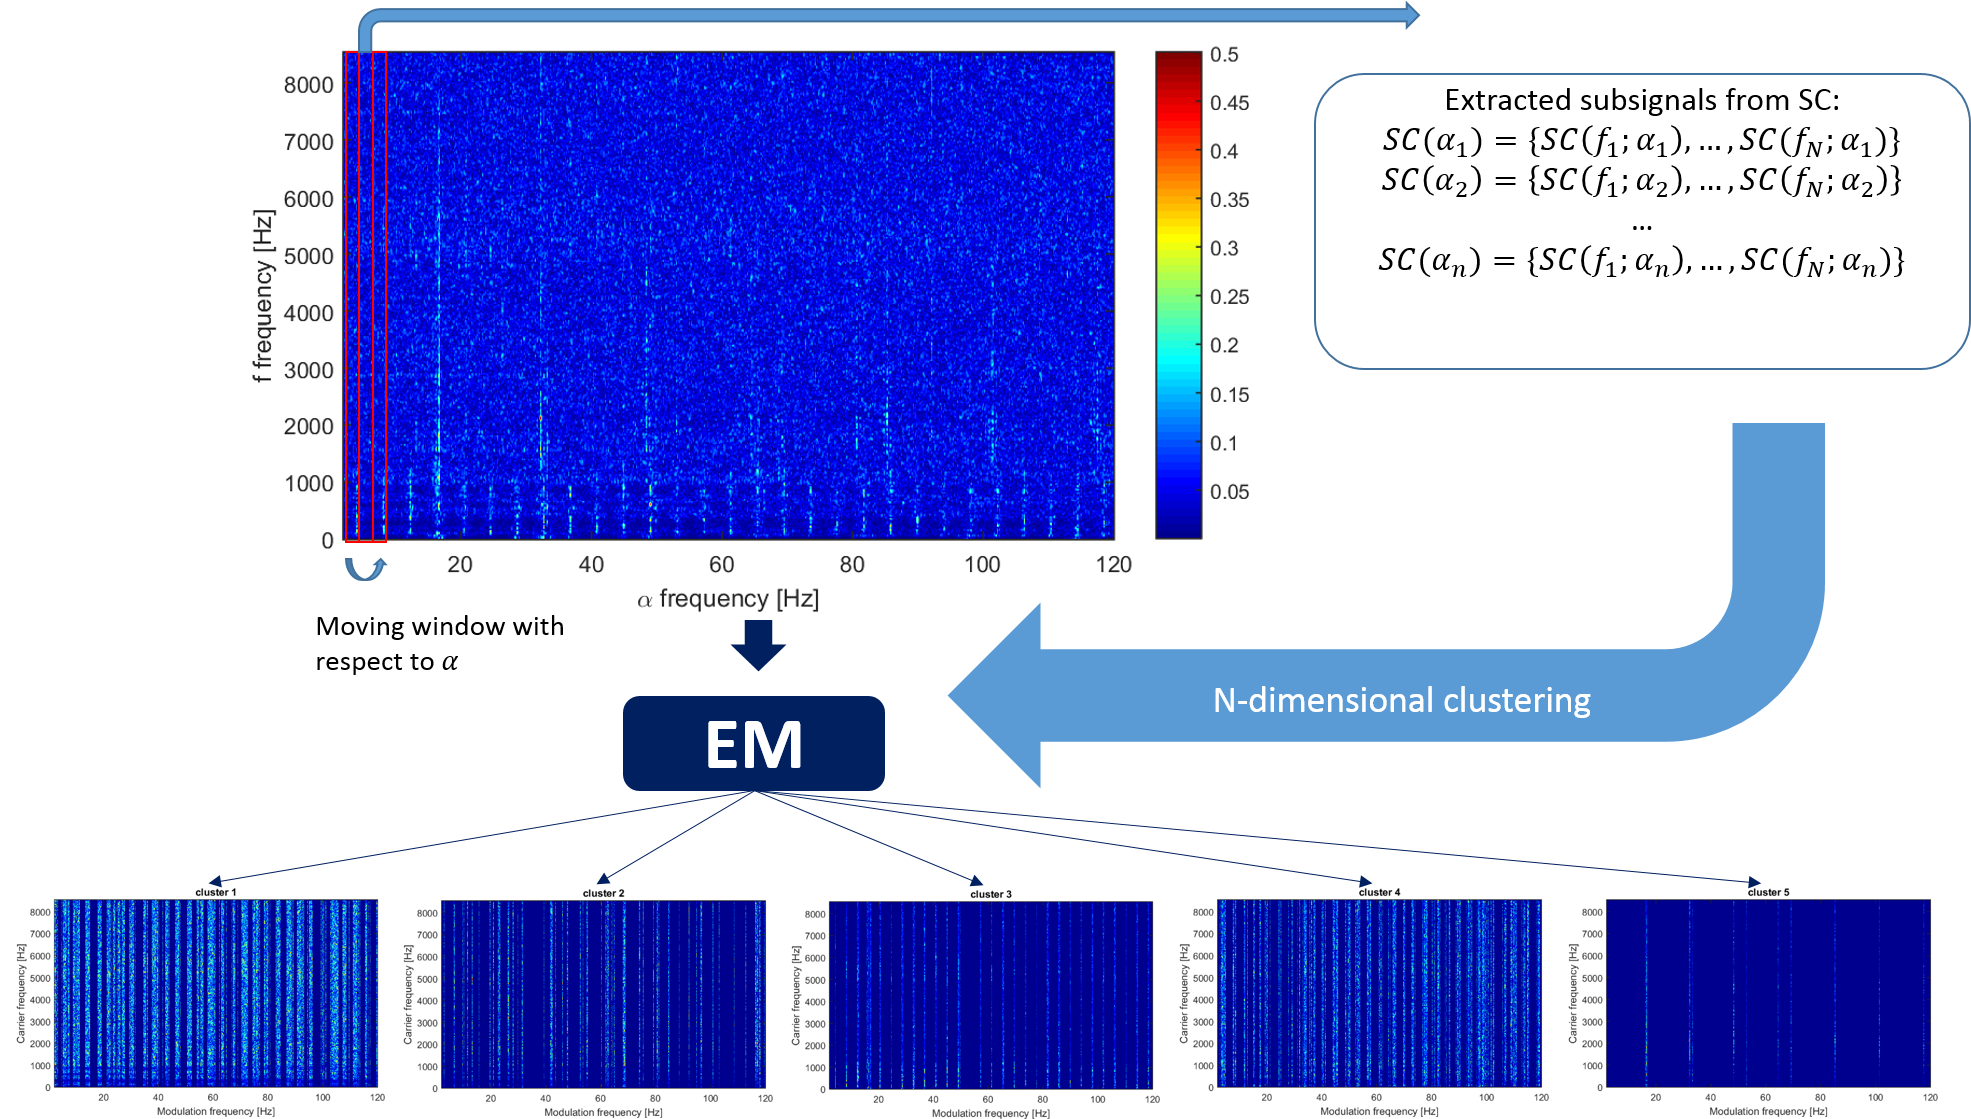
\includegraphics[width=\textwidth]{wykresy/schemat1.png}
\caption{The schema of CSC map clustering.}
\label{fig:clustering}
\end{center}
\end{figure}
In the first step the CSC map is computed for given signal. Therefore the two dimensional function of modulation and carrier frequencies is obtained. Let us assume that size of CSC is $N \times n$.  Then, we extract the subsignals from the map. For instance, for given i-th modulation frequency $\alpha_i$ the following one dimensional function $SC(\alpha_i)=\{SC(f_1;\alpha_i),\dots ,SC(f_1;\alpha_i)\}$ are considered. This $N$ dimensional vectors are inputs for EM. In the next step number of clusters have to be fixed. In order to determine to optimal amount of clusters the Silhouette criterion can be used. Each of the subsignals  is assigned to appropriate group using EM. Finally, the CSC can be plotted for each cluster separately. It is expected that cluster contain information about some signal component. 


%
%
\subsection{CSC map integration}
One can observe that, CSC informs about the excitation for given modulation and carrier frequencies. On the other hand, we are also interested in total energy for  given frequency band. In such case,  we can integrate map with respect to carrier frequency and given modulation frequency \cite{randall2001relationship}. Therefore, the following formula for integrated  CSC in frequency band $[f_1,f_2]$ can be introduced:
\begin{align}
 ISC(\alpha;f_1,f_2)=\sum_{f=f_1}^{f_2}\left|SC(\alpha,f)\right|,
\end{align}
where $\alpha$ is a modulation frequency bin. The one dimension function of modulation frequency is obtained. Therefore, integrated map is significantly higher than zero for cyclostationary signal. Furthermore, it is also related to the the well-known envelope spectrum.

\section{Application}
\label{sec:application}
In this section it is described the application of the proposed methodology for the real data. The signal acquired on the belt conveyor's gearbox is analyzed. It is a two stage gearbox, with the first bevel stage and second spur. The machine is located the underground copper mine. The operational conditions are harsh and the signal is highly contaminated. In Fig. \ref{fig:raw_signal} the raw signal is presented. Its length is equal to 10 seconds and the sampling frequency is 17066~Hz and the frequency of the first shaft is around 16.5 Hz.

\begin{figure}[h!]
\begin{center}
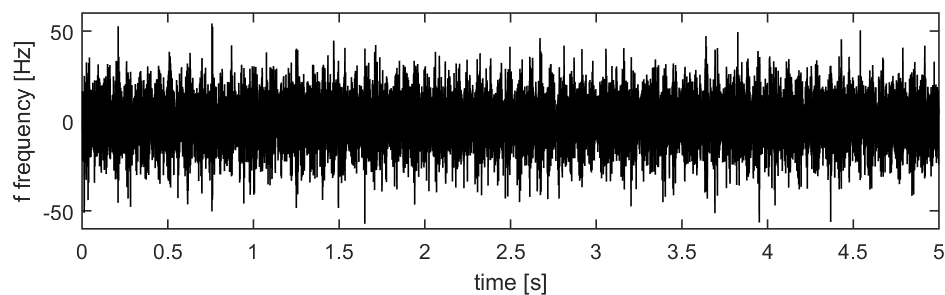
\includegraphics[width=\textwidth]{wykresy/_sygnal.png}
\caption{The raw vibration signal measured on the belt conveyor's gearbox.}
\label{fig:raw_signal}
\end{center}
\end{figure}
The analyzed machine contains two different faults one the first and second shaft. Their fault frequencies are 16.5~Hz  4.17~Hz and respectively. Therefore, it is expected that we are going to obtain the separate clusters for this faults. In the first step the CSC is computed (Fig. \ref{fig:SC}). One can observe that cyclic excitation reveals for low carrier frequencies, with modulation frequency around 4.1 Hz. Furthermore, the wide range excitation can be observed for modulation frequencies around 16.5 Hz and its multiples. The SC for the raw signal is presented in Fig. \ref{fig:SC}. One can observe that there are cyclic excitations for modulation frequency around 16.5 Hz and for 4.1 Hz. Therefore, the SC contain the information about both local damages in the analyzed machine.
%
\begin{figure}[h!]
\begin{center}
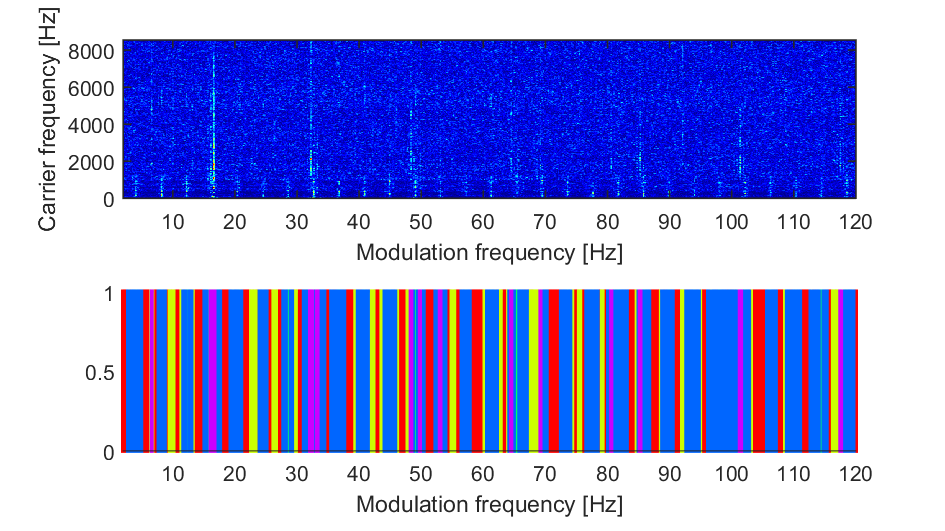
\includegraphics[width=\textwidth]{wykresy/212_SC_clusters.png}
\caption{The Spectral coherence map (upper panel) and the assigned clusters from EM (bottom panel).}
\label{fig:SC}
\end{center}
\end{figure}
%
In order to automatically separate the information for both damages we would like to cluster the SC map using EM method. In case of the clustering it is especially important to use the appropriate number of clusters. Using the Silhouette criterion for determination of cluster numbers was used. As the results the 5 clusters are considered. The assigned cluster are presented in Fig. \ref{fig:SC}. Each cluster is marked with specified color. One can observe, each local damage is assigned to different cluster. Furthermore, these clusters contain only the components related to local faults. 
In further analysis, we are going to considered only clusters no 3 and no 5, which contain information about the damages. 
Therefore, reconstructed based on theses clusters SC maps are presented separately. In Fig. \ref{fig: SC_cluster3} the map containing the information about the damage on the second shaft (4.1~Hz) is presented. The energy is concentrated for low carrier frequency band up to around 1500~Hz.
%
\begin{figure}[h!]
\begin{center}
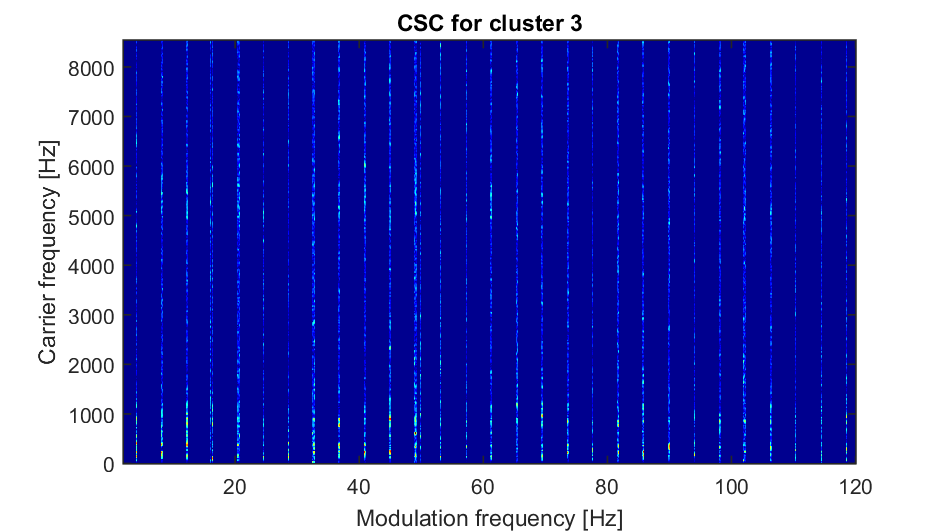
\includegraphics[width=\textwidth]{wykresy/212_SC_cluster_3.png}
\caption{The Spectral coherence map for cluster containing information about the damage on the second shaft.}
\label{fig: SC_cluster3}
\end{center}
\end{figure}
%
The SC map for cluster contain damage for first shaft (16.5~Hz) is presented in Fig. \ref{fig:SC_cluster5}. In this case the wide band excitations are obtained. 
\begin{figure}[h!]
\begin{center}
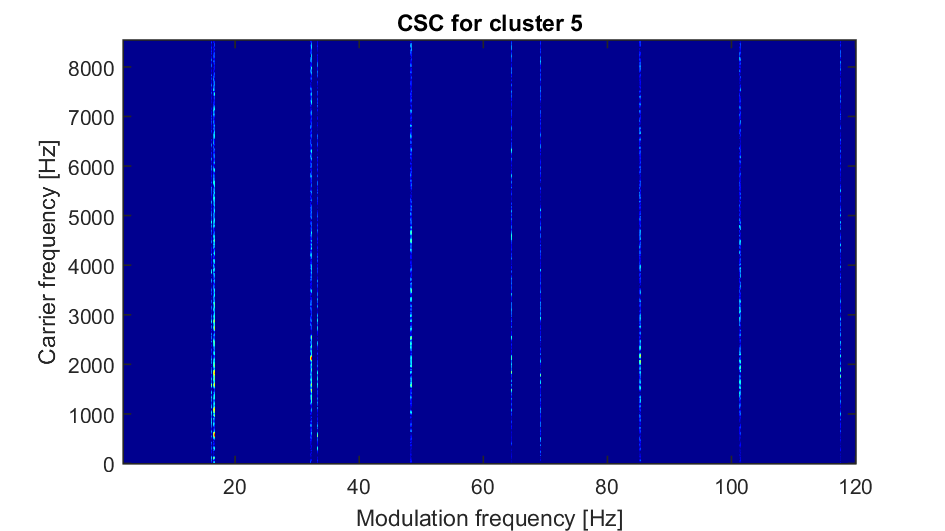
\includegraphics[width=\textwidth]{wykresy/212_SC_cluster_5.png}
\caption{The Spectral coherence map for cluster containing information about the damage on the first shaft.}
\label{fig:SC_cluster5}
\end{center}
\end{figure}
%
Finally the integrated maps for cluster no 3 and no 5 are computed. In Fig. \ref{fig:intSC3} the integrated SC for the cluster containing information about damage for second shaft is presented. One can observe that the excitation for 4.1~Hz and its multiples are observed. 
\begin{figure}[h!]
\begin{center}
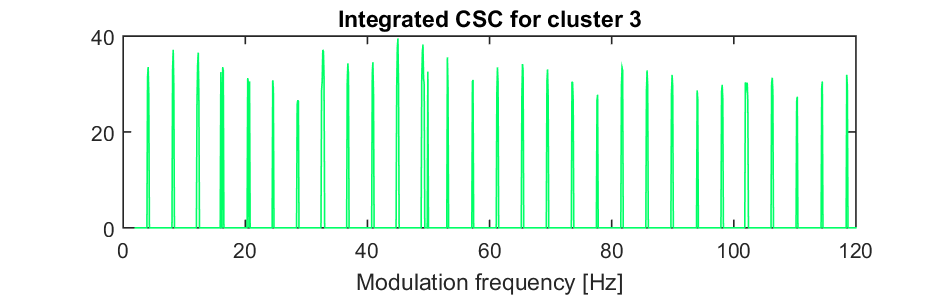
\includegraphics[width=\textwidth]{wykresy/212_cluster_sum_3.png}
\caption{The integrated Spectral coherence map for cluster containing information about the damage on the second shaft.}
\label{fig:intSC3}
\end{center}
\end{figure}
In Fig. \ref{fig:intSC5} the integrated map for cluster no 5 is presented. In this case it contain the information about the damage of the first shaft. In the figure we observe the excitation for 16.5~Hz and its multiples. Therefore, one can observe only the signal component related to the local damage of gear for the first shaft.
\begin{figure}[h!]
\begin{center}
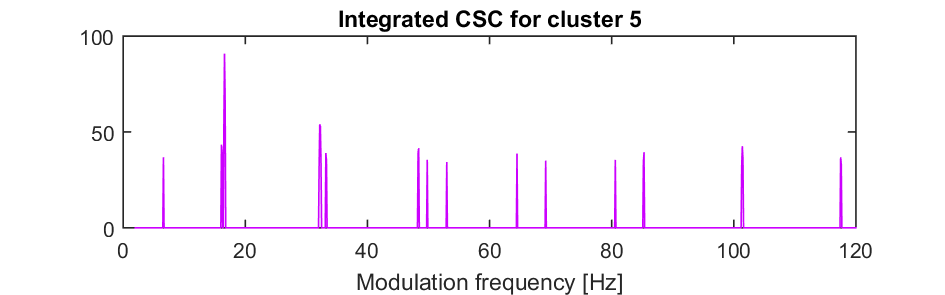
\includegraphics[width=\textwidth]{wykresy/212_cluster_sum_5.png}
\caption{The integrated Spectral coherence map for cluster containing information about the damage on the first shaft.}
\label{fig:intSC5}
\end{center}
\end{figure}

The presented results show that we are able to automatically cluster the SC map and extract the information about several damages. It is worth mentioning that, the usage of appropriate number of clusters is crucial. Each of the signal components should be assigned to a different cluster. Indeed, in the analyzed signal we were able to automatically create two clusters containing the components related to two different local damages. 
\newpage
\section{Summary}
In this article the bi-frequency cyclostationary map was considered. The well known spectral coherence was computed in order to extract information about the local damage in the vibration signal. It is a powerful tool for condition monitoring of the rotating machinery. However, it is mainly analyzed visually, in case of signals with many different cyclic components its interpretation can be challenging. Therefore, it was proposed to apply the automatic method for its clustering. Indeed, EM method was used to cluster the different subsignals from SC. This methodology was tested on real vibration data gathered on belt conveyor. This machine is located in the underground copper mine and it is operating in harsh condition. The analyzed belt conveyor had two damages of  gears (for the first and the second shaft). It was shown that proposed method is able to automatically assign the information about separate local damages to different clusters. 

% \begin{figure}[t]
% \begin{center}
% 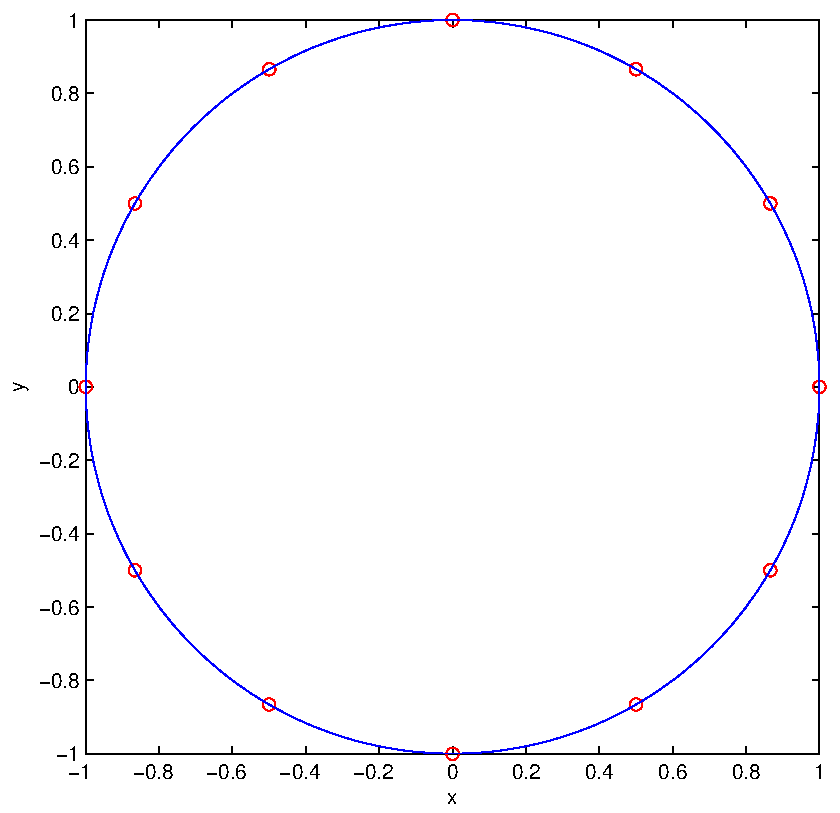
\includegraphics[width=80mm]{circle_rgb}
% \caption{$x = \cos \phi$ and $y = \sin \phi$ \label{f:circle}}
% \end{center}
% \end{figure}

% \begin{table}[ht]
% \centering
% \begin{tabular}{c|cc}
% $\phi$   & $x = \cos \phi$ & $y = \sin \phi$ \\
% \hline
% $0$      &    $1$          &    $0$          \\
% $\pi/6$  &  $\sqrt{3}/2$   &    $1/2$        \\
% $\pi/3$  &    $1/2$        &  $\sqrt{3}/2$   \\
% $\pi/2$  &    $0$          &    $1$
% \end{tabular}
% \caption{Quarter of a circle \label{t:circle}}
% \end{table}




\section*{Acknowledgements}
\bibliographystyle{ISMA}
\bibliography{mybib}

% \begin{thebibliography}{1}

% \bibitem{heylen}
%   W. Heylen, S. Lammens, P. Sas,
%   \textit{Modal Analysis Theory and Testing},
%   Katholieke Universiteit Leuven, Departement Werktuigkunde, Leuven (1997).

% \bibitem{sas}
%   P. Sas, C. Bao, F. Augusztinovicz, W. Desmet,
%   \textit{Active control of sound transmission through a double panel partition},
%   Journal of Sound and Vibration, Vol. 180, No. 4, Academic Press (1995), pp. 609-625.

% \bibitem{boonen}
%   R. Boonen, P. Sas,
%   \textit{Modified Smith Compensation for Feedback Active Noise Control in Ducts},
%   in \mbox{R. Boone}, editor,
%   \textit{Proceedings of The 2001 International Congress and Exhibition
%       on Noise Control Engineering, The Hague, The Netherlands, 2001 August 27-30},
%   The Hague (2001), pp. 619-624.
% \end{thebibliography}




\end{document}
